\section{Solution}

\subsection{Analysis on the Conflicts}

\begin{frame}
	1. Analysis to detect conflicts
	\begin{itemize}
		\item Possible combinations introducing conflicts
		\linebreak
			\begin{figure}
			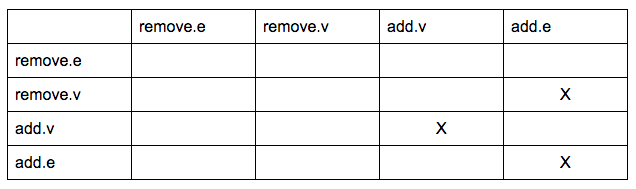
\includegraphics[width=0.8\linewidth]{figures/table.jpg}
			\caption{Combination that creates conflicts}
			\end{figure}
	\end{itemize}
\end{frame}

\begin{frame}	
		 \begin{itemize}
		      \item Refinement of the analysis
		      \linebreak
		   	  \begin{itemize}
				\item Look at the compute() of active vertices in a Superstep 
				\item Collect topology mutation operations
				\item Prune the list if the operation in consideration does not fall into any categories that create conflicts
				\item Take control and data flow into consideration
				\item Formally model the graph mutation and use a proof assistant to prove the correctness of the process
		     	  \end{itemize}
		  \end{itemize}
\end{frame}

\begin{frame}[fragile]
\begin{lstlisting}[
    language=Java]
  Public class SimpleMutateGraphComputation extends BasicComputation<
    LongWritable, DoubleWritable, FloatWritable, DoubleWritable> {

    public void compute(Vertex<LongWritable, DoubleWritable, FloatWritable>
      vertex, Iterable<DoubleWritable> messages){ 
      if (getSuperstep() == 0) {
      	addVertexRequest(getVertexCount(), new
      	DoubleWritable(vertex.getValue()));
      } else if (getSuperstep() == 1) {
        vertex.voteToHalt();
    } 
  }
\end{lstlisting}
Example of a program that mutates a graph
\end{frame}

\begin{frame}	

2. Handle conflicts by abstraction
		      \linebreak
		   	  \begin{itemize}
				\item There are some conflicts that can not be solved by partial ordering 
				\item User defined handlers are suggested to resolve such issues.
				\item Current mechanism is writing user defined handlers to randomly select one of the operation that introduces conflicts.
				\item A better abstraction can add priority to handlers to help decide the operation to be performed if there is a conflict.
		     	  \end{itemize}

\end{frame}


